%sudo apt install libboost-all-dev
%sudo apt install libcurlpp-dev
%sudo apt install libcurl4-openssl-dev
%sudo apt install libssl-dev
%sudo apt install uuid-dev
%https://github.com/beniz/deepdetect/issues/126
%https://github.com/Azure/azure-iot-sdk-c/blob/master/doc/devbox_setup.md
%https://github.com/Azure/azure-iot-sdk-c/blob/master/doc/ubuntu_apt-get_sample_setup.md
%https://www.rti.com/gettingstarted/installlinux_secure
%https://unix.stackexchange.com/questions/389156/how-to-fix-held-broken-packages/389170

\LoadClass[a4paper]{article}
\documentclass{article}

\usepackage{listings}
\lstset{
basicstyle=\ttfamily,
columns=flexible,
breaklines=true
}

\usepackage{verbatim}


\usepackage[hidelinks]{hyperref}
\hypersetup{
	colorlinks=true,
    pdfborder={0 0 0},
    urlcolor     = blue, %Colour for external hyperlinks
    linkcolor    = blue, %Colour of internal links
    citecolor   = red %Colour of citations
}

\usepackage{titlesec}
\newcommand{\sectionbreak}{\clearpage}

\usepackage{graphicx}

\author{Janos Benjamin Antal}
\title{CPS Humidity Homework}
\begin{document}
\maketitle
\section{Prerequisites}
To build the application on Linux Mint 18.3 the following steps are needed:

\begin{itemize}
\item Install required packages with apt: 
\begin{itemize}
\item \verb+libboost-all-dev+
\item \verb+libcurl4-openssl-dev+
\item \verb+libssl-dev+ %(some help can be found \href{https://unix.stackexchange.com/a/389170}{here})
\item \verb+uuid-dev+
\item \verb+rapidjson-dev+
\item \verb+build-essential+
\item \verb+cmake+
\item \verb!g++!
\item \verb+git+
\end{itemize}
Use the following command:
\begin{lstlisting}
$ sudo apt install libboost-all-dev libcurl4-openssl-dev libssl-dev uuid-dev rapidjson-dev build-essential cmake g++ git
\end{lstlisting}
\item Install \href{http://www.curlpp.org/}{cURLpp} with the steps described \href{https://github.com/beniz/deepdetect/issues/126}{here}:
\begin{verbatim}
$ sudo apt-get remove libcurlpp0
$ mkdir curlppbuild
$ cd curlppbuild
$ git clone https://github.com/jpbarrette/curlpp.git
$ cd curlpp
$ cmake .
$ sudo make install
\end{verbatim} 
%\item Install \href{http://rapidjson.org/}{RapidJSON} with the steps described \href{https://github.com/Tencent/rapidjson}{here}. Unfortunately, RapidJSON can be compiled with GNU C++ compiler 5.4.0 because of a strange warning is interpreted as error. I already created an issue about it in github. Until this going to be fixed, just remove \verb!-Weffc++! from \verb+CMakeList.txt+. 
%\begin{verbatim}
%$ mkdir rapidjsonbuild
%$ cd rapidjsonbuild
%$ git clone https://github.com/Tencent/rapidjson.git
%$ cd rapidjson
%$ git submodule update --init
%$ mkdir build
%$ cd build
%$ cmake ..
%$ sudo make install
%\end{verbatim} 
\item Install AzureIoT C SDKfrom \href{https://github.com/Azure/azure-iot-sdk-c/blob/master/doc/devbox_setup.md}{source}. After building the SDK use \verb+sudo make install+ to copy the header and the lib files to the system include path.
\item Download and install \href{https://www.rti.com/gettingstarted/installlinux_secure}{RTI Connext DDS 5.3}
\item Set the \verb+NDDSHOME+ environment variable to the root of RTI Connext DDS, e.g.: \verb+/opt/rti_connext_dds-5.3.0+
\end{itemize}

\section{Build}
\begin{enumerate}
\item Clone git repository
\begin{lstlisting}
$ git clone https://github.com/antaljanosbenjamin/cps_homework.git
\end{lstlisting}
\item Generate source code from .idl files
\begin{lstlisting}[language=bash]
$ cd cps_homework
$ $NDDSHOME/bin/rtiddsgen  -language C++11 -stl -d DDS/Config/common -replace idl_files/Config.idl
$ $NDDSHOME/bin/rtiddsgen  -language C++11 -stl -d DDS/Decision/common -replace idl_files/Decision.idl
$ $NDDSHOME/bin/rtiddsgen  -language C++11 -stl -d DDS/Schedule/common -replace idl_files/Schedule.idl
$ $NDDSHOME/bin/rtiddsgen  -language C++11 -stl -d DDS/Humidity/common -replace idl_files/UvegHaz.idl
$ $NDDSHOME/bin/rtiddsgen  -language C++11 -stl -d DDS/Weather/common -replace idl_files/Weather.idl
\end{lstlisting}
\item Build
\begin{lstlisting}
$ mkdir build
$ cd build
$ cmake ..
$ make [-j 8]
\end{lstlisting}
\end{enumerate}

\section{Run demo}
\begin{enumerate}
\item Start humidity publisher
\begin{verbatim}
$ ./cps_main h <humidityDataFilePath>
\end{verbatim}
As result of this command the application will read the data file and start to publish a humidity value every 4 minutes. The file shall contains a humidity value per line. Each humidity value is a decimal number. See example \href{https://github.com/antaljanosbenjamin/cps_homework/blob/master/examples/humidity.txt}{file}.
\item Start IoTEdge 
\begin{lstlisting}
$ ./cps_main e <weatherApiKey> <azureConnectionString> <scheduleFilePath>
\end{lstlisting} 
The meaning of parameteres are the following:
\begin{itemize}
\item \verb+weatherApiKey+: an API key for http://api.airvisual.com
\item \verb+azureConnectionString+: the connection string of the device used Azure IoT Hub
\item \verb+scheduleFilePath+: path to a CSV file which stores the schedules time intervals. See example \href{https://github.com/antaljanosbenjamin/cps_homework/blob/master/examples/schedule.csv}{file}.
\end{itemize}
The IoTEdge module is responsible to communicate with Azure IoT Hub, the weather information system and also to send schedule information through DDS topic.
\item Start humidity controller
\begin{verbatim}
$ ./cps_main c
\end{verbatim}
The controller receives the required informations and sensor values and also make decisions based on the collected data. It also sends the decision input and output to the IoTEdge in order to store them in the cloud.
\end{enumerate}
\section{System architecture}
The system consists three modules:
\begin{itemize}
\item IoTEdge
\item Controller
\item Publisher
\end{itemize}
The publisher module exists only for testing purposes, so this documentation doesn't contains it's details.
\subsection{IoTEdge}
\begin{figure}[!htb]
  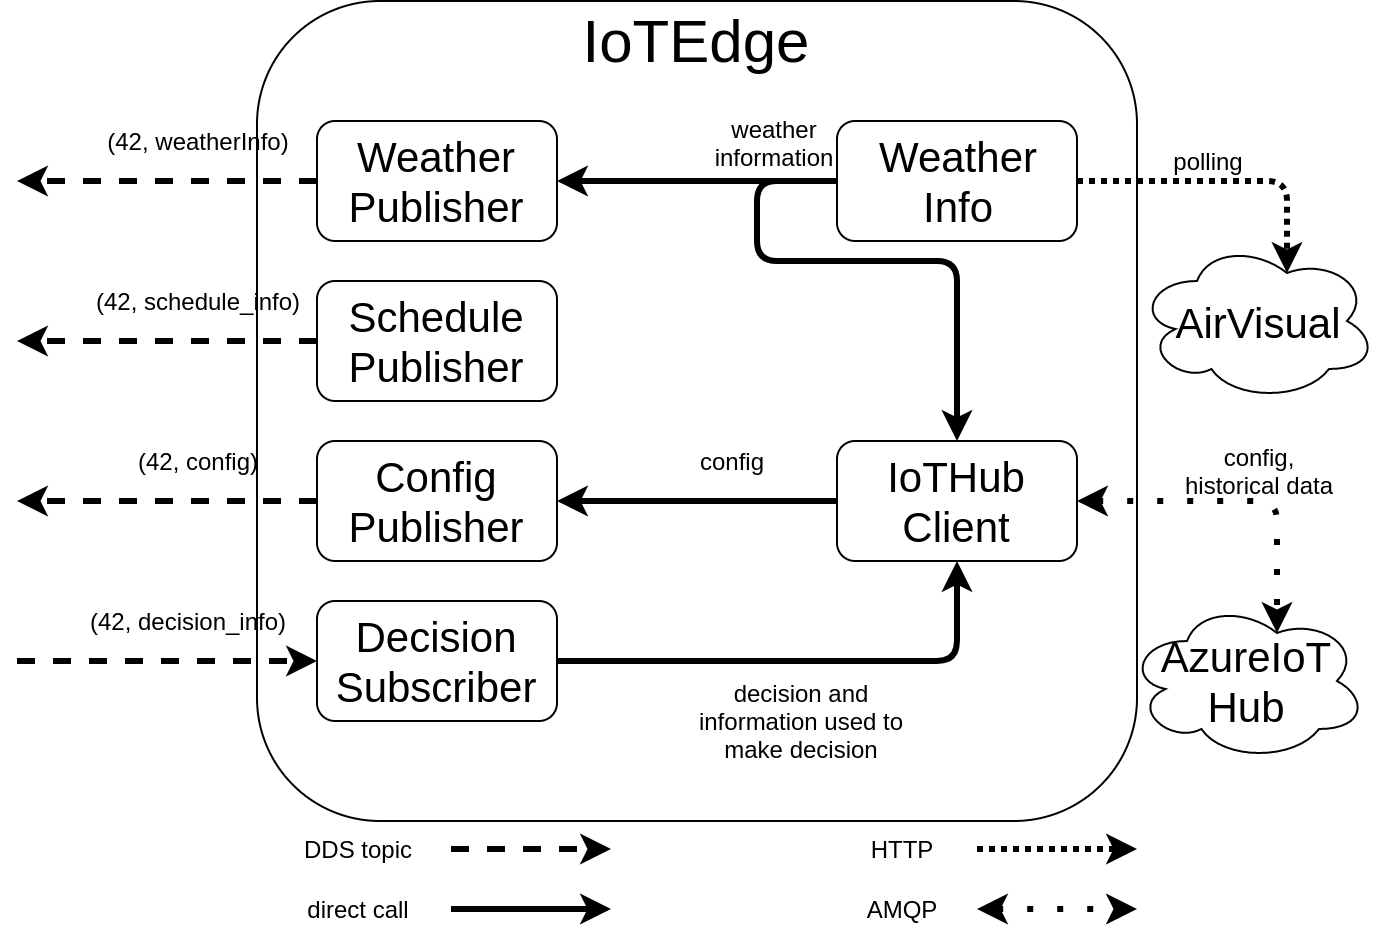
\includegraphics[width=\linewidth]{imgs/edge.png}
  \caption{Architecture of IoT Edge}
  \label{fig:arc_edge}
\end{figure}

Figure \ref{fig:arc_edge} shows the semantic architecture of IoT Edge. 

\end{document}